\documentclass{standalone}
\usepackage{tikz}
\usetikzlibrary{patterns, positioning}


\begin{document}
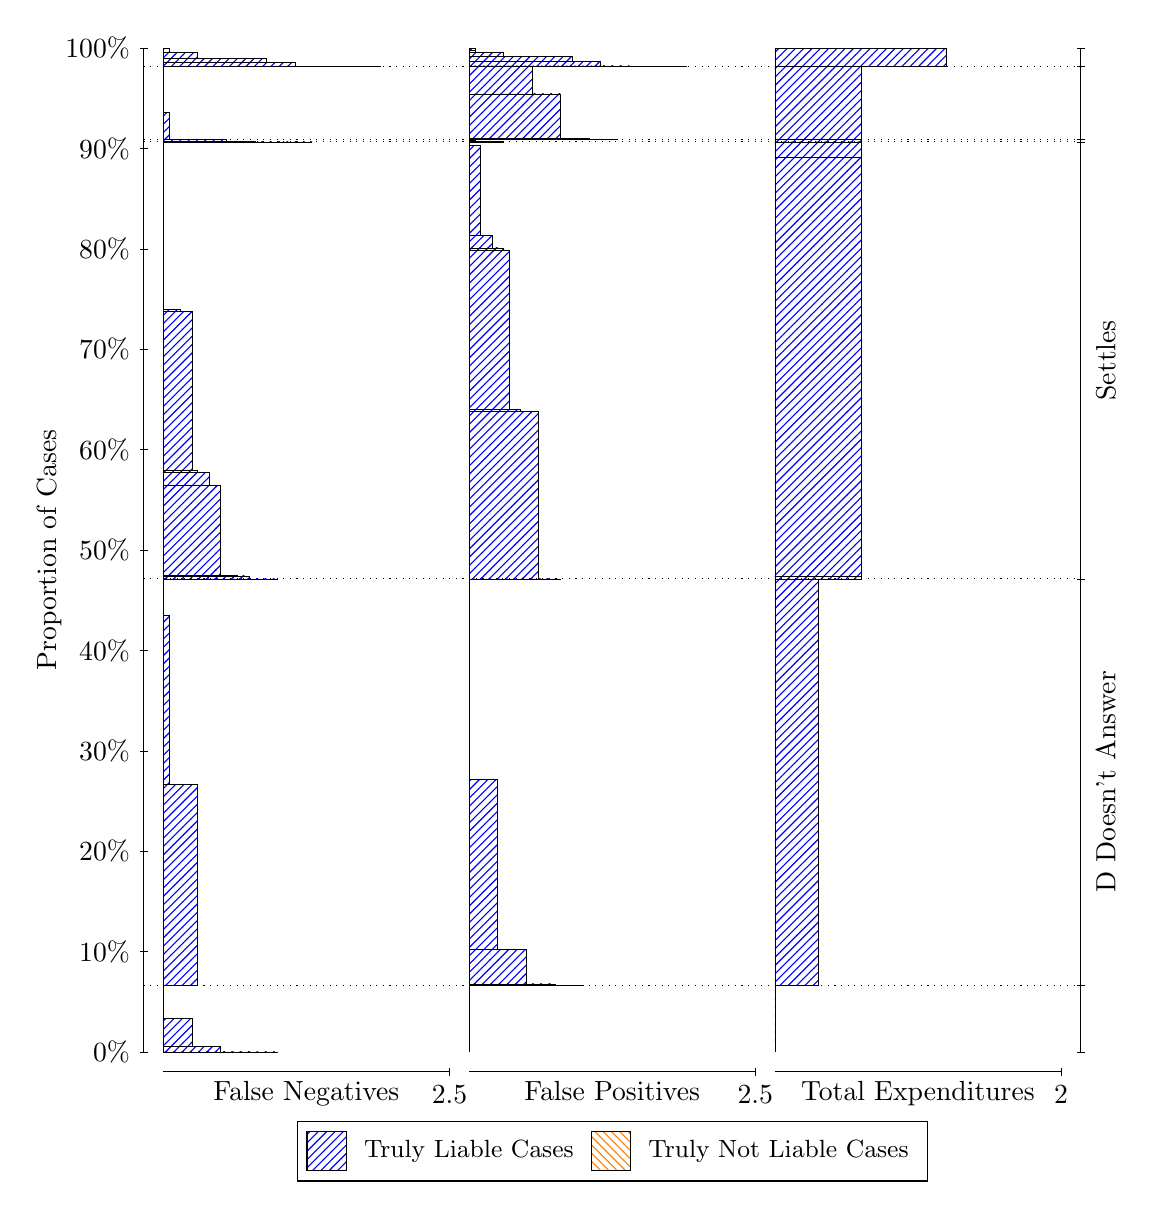
\begin{tikzpicture}
\draw[black, very thin] (1.5,1.75) -- (1.5,14.5);
\node[rotate=90, text=black, anchor=center] at (0.3, 8.125) {Proportion of Cases};
\draw[black, very thin] (1.45,1.75) -- (1.55,1.75);
\node[text=black, anchor=east] at (1.45, 1.75) {0\%};
\draw[black, very thin] (1.45,3.025) -- (1.55,3.025);
\node[text=black, anchor=east] at (1.45, 3.025) {10\%};
\draw[black, very thin] (1.45,4.3) -- (1.55,4.3);
\node[text=black, anchor=east] at (1.45, 4.3) {20\%};
\draw[black, very thin] (1.45,5.575) -- (1.55,5.575);
\node[text=black, anchor=east] at (1.45, 5.575) {30\%};
\draw[black, very thin] (1.45,6.85) -- (1.55,6.85);
\node[text=black, anchor=east] at (1.45, 6.85) {40\%};
\draw[black, very thin] (1.45,8.125) -- (1.55,8.125);
\node[text=black, anchor=east] at (1.45, 8.125) {50\%};
\draw[black, very thin] (1.45,9.4) -- (1.55,9.4);
\node[text=black, anchor=east] at (1.45, 9.4) {60\%};
\draw[black, very thin] (1.45,10.675) -- (1.55,10.675);
\node[text=black, anchor=east] at (1.45, 10.675) {70\%};
\draw[black, very thin] (1.45,11.95) -- (1.55,11.95);
\node[text=black, anchor=east] at (1.45, 11.95) {80\%};
\draw[black, very thin] (1.45,13.225) -- (1.55,13.225);
\node[text=black, anchor=east] at (1.45, 13.225) {90\%};
\draw[black, very thin] (1.45,14.5) -- (1.55,14.5);
\node[text=black, anchor=east] at (1.45, 14.5) {100\%};

\draw[black, very thin] (13.4,1.75) -- (13.4,14.5);
\draw[black, very thin] (13.35,1.75) -- (13.45,1.75);
\node[anchor=west] at (13.35, 1.75) {};
\draw[black, very thin] (13.35,2.5998) -- (13.45,2.5998);
\node[anchor=west] at (13.35, 2.5998) {};
\draw[black, very thin] (13.35,7.7595) -- (13.45,7.7595);
\node[anchor=west] at (13.35, 7.7595) {};
\draw[black, very thin] (13.35,13.309) -- (13.45,13.309);
\node[anchor=west] at (13.35, 13.309) {};
\draw[black, very thin] (13.35,13.336) -- (13.45,13.336);
\node[anchor=west] at (13.35, 13.336) {};
\draw[black, very thin] (13.35,14.266) -- (13.45,14.266);
\node[anchor=west] at (13.35, 14.266) {};
\draw[black, very thin] (13.35,14.5) -- (13.45,14.5);
\node[anchor=west] at (13.35, 14.5) {};

\draw[black, very thin, pattern color=blue, pattern=north east lines] (1.75,1.75) rectangle (3.2033,1.75);
\draw[black, very thin, pattern color=blue, pattern=north east lines] (1.75,1.75) rectangle (2.84,1.7506);
\draw[black, very thin, pattern color=blue, pattern=north east lines] (1.75,1.7506) rectangle (2.4767,1.818);
\draw[black, very thin, pattern color=blue, pattern=north east lines] (1.75,1.818) rectangle (2.1133,2.1755);
\draw[black, very thin, pattern color=orange, pattern=north west lines] (1.75,2.1755) rectangle (1.75,2.1755);
\draw[black, very thin, pattern color=blue, pattern=north east lines] (1.75,2.1755) rectangle (1.75,2.5998);
\draw[black, very thin, pattern color=blue, pattern=north east lines] (1.75,2.5998) rectangle (2.186,5.1458);
\draw[black, very thin, pattern color=blue, pattern=north east lines] (1.75,5.1458) rectangle (1.8227,7.3016);
\draw[black, very thin, pattern color=orange, pattern=north west lines] (1.75,7.3016) rectangle (1.75,7.3016);
\draw[black, very thin, pattern color=blue, pattern=north east lines] (1.75,7.3016) rectangle (1.75,7.7595);
\draw[black, very thin, pattern color=blue, pattern=north east lines] (1.75,7.7595) rectangle (3.2033,7.7595);
\draw[black, very thin, pattern color=blue, pattern=north east lines] (1.75,7.7595) rectangle (3.058,7.7595);
\draw[black, very thin, pattern color=blue, pattern=north east lines] (1.75,7.7595) rectangle (2.9127,7.7595);
\draw[black, very thin, pattern color=blue, pattern=north east lines] (1.75,7.7595) rectangle (2.84,7.7968);
\draw[black, very thin, pattern color=blue, pattern=north east lines] (1.75,7.7968) rectangle (2.6947,7.8046);
\draw[black, very thin, pattern color=blue, pattern=north east lines] (1.75,7.8046) rectangle (2.5493,7.8059);
\draw[black, very thin, pattern color=blue, pattern=north east lines] (1.75,7.8059) rectangle (2.4767,8.9436);
\draw[black, very thin, pattern color=blue, pattern=north east lines] (1.75,8.9436) rectangle (2.3313,9.1059);
\draw[black, very thin, pattern color=blue, pattern=north east lines] (1.75,9.1059) rectangle (2.186,9.1331);
\draw[black, very thin, pattern color=blue, pattern=north east lines] (1.75,9.1331) rectangle (2.1133,11.157);
\draw[black, very thin, pattern color=blue, pattern=north east lines] (1.75,11.157) rectangle (1.968,11.181);
\draw[black, very thin, pattern color=blue, pattern=north east lines] (1.75,11.181) rectangle (1.8227,11.185);
\draw[black, very thin, pattern color=orange, pattern=north west lines] (1.75,11.185) rectangle (1.75,11.185);
\draw[black, very thin, pattern color=blue, pattern=north east lines] (1.75,11.185) rectangle (1.75,13.309);
\draw[black, very thin, pattern color=blue, pattern=north east lines] (1.75,13.309) rectangle (3.6393,13.309);
\draw[black, very thin, pattern color=blue, pattern=north east lines] (1.75,13.309) rectangle (3.276,13.309);
\draw[black, very thin, pattern color=blue, pattern=north east lines] (1.75,13.309) rectangle (2.9127,13.319);
\draw[black, very thin, pattern color=blue, pattern=north east lines] (1.75,13.319) rectangle (2.5493,13.336);
\draw[black, very thin, pattern color=blue, pattern=north east lines] (1.75,13.336) rectangle (2.186,13.336);
\draw[black, very thin, pattern color=orange, pattern=north west lines] (1.75,13.336) rectangle (1.75,13.336);
\draw[black, very thin, pattern color=blue, pattern=north east lines] (1.75,13.336) rectangle (2.186,13.34);
\draw[black, very thin, pattern color=blue, pattern=north east lines] (1.75,13.34) rectangle (1.8227,13.685);
\draw[black, very thin, pattern color=orange, pattern=north west lines] (1.75,13.685) rectangle (1.75,13.685);
\draw[black, very thin, pattern color=blue, pattern=north east lines] (1.75,13.685) rectangle (1.75,14.266);
\draw[black, very thin, pattern color=blue, pattern=north east lines] (1.75,14.266) rectangle (4.5113,14.266);
\draw[black, very thin, pattern color=blue, pattern=north east lines] (1.75,14.266) rectangle (4.148,14.266);
\draw[black, very thin, pattern color=blue, pattern=north east lines] (1.75,14.266) rectangle (3.7847,14.27);
\draw[black, very thin, pattern color=blue, pattern=north east lines] (1.75,14.27) rectangle (3.4213,14.322);
\draw[black, very thin, pattern color=blue, pattern=north east lines] (1.75,14.322) rectangle (3.276,14.322);
\draw[black, very thin, pattern color=blue, pattern=north east lines] (1.75,14.322) rectangle (3.058,14.371);
\draw[black, very thin, pattern color=blue, pattern=north east lines] (1.75,14.371) rectangle (2.9127,14.371);
\draw[black, very thin, pattern color=blue, pattern=north east lines] (1.75,14.371) rectangle (2.6947,14.371);
\draw[black, very thin, pattern color=blue, pattern=north east lines] (1.75,14.371) rectangle (2.5493,14.373);
\draw[black, very thin, pattern color=blue, pattern=north east lines] (1.75,14.373) rectangle (2.3313,14.373);
\draw[black, very thin, pattern color=blue, pattern=north east lines] (1.75,14.373) rectangle (2.186,14.373);
\draw[black, very thin, pattern color=blue, pattern=north east lines] (1.75,14.373) rectangle (2.186,14.441);
\draw[black, very thin, pattern color=blue, pattern=north east lines] (1.75,14.441) rectangle (1.8227,14.442);
\draw[black, very thin, pattern color=blue, pattern=north east lines] (1.75,14.442) rectangle (1.8227,14.495);
\draw[black, very thin, pattern color=orange, pattern=north west lines] (1.75,14.495) rectangle (1.75,14.495);
\draw[black, very thin, pattern color=blue, pattern=north east lines] (1.75,14.495) rectangle (1.75,14.5);
\draw[black, very thin, pattern color=orange, pattern=north west lines] (5.6333,1.75) rectangle (5.6333,1.75);
\draw[black, very thin, pattern color=blue, pattern=north east lines] (5.6333,1.75) rectangle (5.6333,2.5998);
\draw[black, very thin, pattern color=orange, pattern=north west lines] (5.6333,2.5998) rectangle (7.0867,2.5998);
\draw[black, very thin, pattern color=blue, pattern=north east lines] (5.6333,2.5998) rectangle (7.0867,2.5999);
\draw[black, very thin, pattern color=blue, pattern=north east lines] (5.6333,2.5999) rectangle (6.7233,2.6143);
\draw[black, very thin, pattern color=blue, pattern=north east lines] (5.6333,2.6143) rectangle (6.36,3.0577);
\draw[black, very thin, pattern color=blue, pattern=north east lines] (5.6333,3.0577) rectangle (5.9967,5.2135);
\draw[black, very thin, pattern color=blue, pattern=north east lines] (5.6333,5.2135) rectangle (5.6333,7.7595);
\draw[black, very thin, pattern color=orange, pattern=north west lines] (5.6333,7.7595) rectangle (6.796,7.7595);
\draw[black, very thin, pattern color=blue, pattern=north east lines] (5.6333,7.7595) rectangle (6.796,7.7595);
\draw[black, very thin, pattern color=orange, pattern=north west lines] (5.6333,7.7595) rectangle (6.6507,7.7595);
\draw[black, very thin, pattern color=blue, pattern=north east lines] (5.6333,7.7595) rectangle (6.6507,7.7595);
\draw[black, very thin, pattern color=orange, pattern=north west lines] (5.6333,7.7595) rectangle (6.5053,7.7595);
\draw[black, very thin, pattern color=blue, pattern=north east lines] (5.6333,7.7595) rectangle (6.5053,9.8834);
\draw[black, very thin, pattern color=blue, pattern=north east lines] (5.6333,9.8834) rectangle (6.4327,9.8875);
\draw[black, very thin, pattern color=blue, pattern=north east lines] (5.6333,9.8875) rectangle (6.2873,9.9117);
\draw[black, very thin, pattern color=blue, pattern=north east lines] (5.6333,9.9117) rectangle (6.142,11.935);
\draw[black, very thin, pattern color=blue, pattern=north east lines] (5.6333,11.935) rectangle (6.0693,11.963);
\draw[black, very thin, pattern color=blue, pattern=north east lines] (5.6333,11.963) rectangle (5.924,12.125);
\draw[black, very thin, pattern color=blue, pattern=north east lines] (5.6333,12.125) rectangle (5.7787,13.263);
\draw[black, very thin, pattern color=blue, pattern=north east lines] (5.6333,13.263) rectangle (5.706,13.264);
\draw[black, very thin, pattern color=blue, pattern=north east lines] (5.6333,13.264) rectangle (5.6333,13.309);
\draw[black, very thin, pattern color=orange, pattern=north west lines] (5.6333,13.309) rectangle (6.0693,13.309);
\draw[black, very thin, pattern color=blue, pattern=north east lines] (5.6333,13.309) rectangle (6.0693,13.31);
\draw[black, very thin, pattern color=blue, pattern=north east lines] (5.6333,13.31) rectangle (5.706,13.327);
\draw[black, very thin, pattern color=blue, pattern=north east lines] (5.6333,13.327) rectangle (5.6333,13.336);
\draw[black, very thin, pattern color=orange, pattern=north west lines] (5.6333,13.336) rectangle (7.5227,13.336);
\draw[black, very thin, pattern color=blue, pattern=north east lines] (5.6333,13.336) rectangle (7.5227,13.336);
\draw[black, very thin, pattern color=blue, pattern=north east lines] (5.6333,13.336) rectangle (7.1593,13.353);
\draw[black, very thin, pattern color=blue, pattern=north east lines] (5.6333,13.353) rectangle (6.796,13.918);
\draw[black, very thin, pattern color=blue, pattern=north east lines] (5.6333,13.918) rectangle (6.4327,14.263);
\draw[black, very thin, pattern color=blue, pattern=north east lines] (5.6333,14.263) rectangle (6.0693,14.266);
\draw[black, very thin, pattern color=orange, pattern=north west lines] (5.6333,14.266) rectangle (8.3947,14.266);
\draw[black, very thin, pattern color=blue, pattern=north east lines] (5.6333,14.266) rectangle (8.3947,14.266);
\draw[black, very thin, pattern color=orange, pattern=north west lines] (5.6333,14.266) rectangle (8.0313,14.266);
\draw[black, very thin, pattern color=blue, pattern=north east lines] (5.6333,14.266) rectangle (8.0313,14.267);
\draw[black, very thin, pattern color=orange, pattern=north west lines] (5.6333,14.267) rectangle (7.668,14.267);
\draw[black, very thin, pattern color=blue, pattern=north east lines] (5.6333,14.267) rectangle (7.668,14.272);
\draw[black, very thin, pattern color=orange, pattern=north west lines] (5.6333,14.272) rectangle (7.3047,14.272);
\draw[black, very thin, pattern color=blue, pattern=north east lines] (5.6333,14.272) rectangle (7.3047,14.326);
\draw[black, very thin, pattern color=blue, pattern=north east lines] (5.6333,14.326) rectangle (6.9413,14.394);
\draw[black, very thin, pattern color=orange, pattern=north west lines] (5.6333,14.394) rectangle (6.796,14.394);
\draw[black, very thin, pattern color=blue, pattern=north east lines] (5.6333,14.394) rectangle (6.796,14.394);
\draw[black, very thin, pattern color=blue, pattern=north east lines] (5.6333,14.394) rectangle (6.578,14.395);
\draw[black, very thin, pattern color=orange, pattern=north west lines] (5.6333,14.395) rectangle (6.4327,14.395);
\draw[black, very thin, pattern color=blue, pattern=north east lines] (5.6333,14.395) rectangle (6.4327,14.395);
\draw[black, very thin, pattern color=blue, pattern=north east lines] (5.6333,14.395) rectangle (6.2147,14.395);
\draw[black, very thin, pattern color=blue, pattern=north east lines] (5.6333,14.395) rectangle (6.0693,14.443);
\draw[black, very thin, pattern color=orange, pattern=north west lines] (5.6333,14.443) rectangle (6.0693,14.443);
\draw[black, very thin, pattern color=blue, pattern=north east lines] (5.6333,14.443) rectangle (6.0693,14.444);
\draw[black, very thin, pattern color=blue, pattern=north east lines] (5.6333,14.444) rectangle (5.8513,14.444);
\draw[black, very thin, pattern color=blue, pattern=north east lines] (5.6333,14.444) rectangle (5.706,14.475);
\draw[black, very thin, pattern color=blue, pattern=north east lines] (5.6333,14.475) rectangle (5.706,14.497);
\draw[black, very thin, pattern color=blue, pattern=north east lines] (5.6333,14.497) rectangle (5.6333,14.5);
\draw[black, very thin, pattern color=orange, pattern=north west lines] (9.5167,1.75) rectangle (9.5167,1.75);
\draw[black, very thin, pattern color=blue, pattern=north east lines] (9.5167,1.75) rectangle (9.5167,2.5998);
\draw[black, very thin, pattern color=orange, pattern=north west lines] (9.5167,2.5998) rectangle (10.062,2.5998);
\draw[black, very thin, pattern color=blue, pattern=north east lines] (9.5167,2.5998) rectangle (10.062,7.7595);
\draw[black, very thin, pattern color=orange, pattern=north west lines] (9.5167,7.7595) rectangle (10.607,7.7595);
\draw[black, very thin, pattern color=blue, pattern=north east lines] (9.5167,7.7595) rectangle (10.607,7.7921);
\draw[black, very thin, pattern color=orange, pattern=north west lines] (9.5167,7.7921) rectangle (10.607,7.7921);
\draw[black, very thin, pattern color=blue, pattern=north east lines] (9.5167,7.7921) rectangle (10.607,13.115);
\draw[black, very thin, pattern color=orange, pattern=north west lines] (9.5167,13.115) rectangle (10.607,13.115);
\draw[black, very thin, pattern color=blue, pattern=north east lines] (9.5167,13.115) rectangle (10.607,13.309);
\draw[black, very thin, pattern color=orange, pattern=north west lines] (9.5167,13.309) rectangle (10.607,13.309);
\draw[black, very thin, pattern color=blue, pattern=north east lines] (9.5167,13.309) rectangle (10.607,13.336);
\draw[black, very thin, pattern color=orange, pattern=north west lines] (9.5167,13.336) rectangle (10.607,13.336);
\draw[black, very thin, pattern color=blue, pattern=north east lines] (9.5167,13.336) rectangle (10.607,14.266);
\draw[black, very thin, pattern color=orange, pattern=north west lines] (9.5167,14.266) rectangle (11.697,14.266);
\draw[black, very thin, pattern color=blue, pattern=north east lines] (9.5167,14.266) rectangle (11.697,14.5);
\draw[black, dotted] (1.5,2.5998) -- (13.4,2.5998);
\draw[black, dotted] (1.5,7.7595) -- (13.4,7.7595);
\draw[black, dotted] (1.5,13.309) -- (13.4,13.309);
\draw[black, dotted] (1.5,13.336) -- (13.4,13.336);
\draw[black, dotted] (1.5,14.266) -- (13.4,14.266);
\draw[black, very thin] (1.75,1.5) -- (5.3833,1.5);
\node[text=black, anchor=north] at (3.5667, 1.5) {False Negatives};
\draw[black, very thin] (5.3833,1.45) -- (5.3833,1.55);
\node[text=black, anchor=north] at (5.3833, 1.45) {2.5};

\draw[black, very thin] (5.6333,1.5) -- (9.2667,1.5);
\node[text=black, anchor=north] at (7.45, 1.5) {False Positives};
\draw[black, very thin] (9.2667,1.45) -- (9.2667,1.55);
\node[text=black, anchor=north] at (9.2667, 1.45) {2.5};

\draw[black, very thin] (9.5167,1.5) -- (13.15,1.5);
\node[text=black, anchor=north] at (11.333, 1.5) {Total Expenditures};
\draw[black, very thin] (13.15,1.45) -- (13.15,1.55);
\node[text=black, anchor=north] at (13.15, 1.45) {2};


\node[text=black, centered, rotate=90] at (13.72, 5.1796) {D Doesn't Answer};
\node[text=black, centered, rotate=90] at (13.72, 10.534) {Settles};




\draw (7.449999999999999,1.5) node[draw=none] (baseCoordinate) {};
\begin{scope}[align=center]
        \matrix[scale=0.5, draw=black, below=0.5cm of baseCoordinate, nodes={draw}, column sep=0.1cm]{
            \node[rectangle, draw, minimum width=0.5cm, minimum height=0.5cm, pattern color=blue, pattern=north east lines] {}; &
            \node[draw=none, font=\small, text=black] (B) {Truly Liable Cases}; &
            \node[rectangle, draw, minimum width=0.5cm, minimum height=0.5cm, pattern color=orange, pattern=north west lines] {}; &
            \node[draw=none, font=\small, text=black] (B) {Truly Not Liable Cases}; \\
            };
\end{scope}

\end{tikzpicture}
\end{document}